\documentclass[
  11pt,
  letterpaper,
   addpoints,
   answers
  ]{exam}

\usepackage[utf8]{inputenc}
\usepackage{../exercise-preamble}
\usepackage{float}
\usepackage{subcaption}
% TikZ libraries needed for `right=.. of ..` and coordinate math

\begin{document}

\noindent
\begin{minipage}{0.47\textwidth}

\includegraphics[width=\textwidth]{../fcfm_die}
\end{minipage}
\begin{minipage}{0.53\textwidth}
\begin{center} 
\large\textbf{Análisis de señales} (EL3203-2) \\
\large\textbf{Clase auxiliar 3} \\
\normalsize Prof.~Jorge Silva.\\
\normalsize Prof.~Aux.~Erik Sáez
\end{center}
\end{minipage}

\vspace{0.5cm}
\noindent
\vspace{.85cm}
%----------------------------
\noindent\rule{\textwidth}{0.4pt}
\subsection*{Serie de Fourier de una señal $T$-periódica}
La serie de Fourier permite descomponer cualquier señal periódica en una suma de funciones sinusoidales (armónicos) de distintas frecuencias, amplitudes y fases. Cada armónico tiene una frecuencia múltiplo de la fundamental $\omega_0=\tfrac{2\pi}{T}$, donde $T$ es el período de la señal. Así, cualquier señal $T$-periódica se puede escribir como:
\begin{equation}
  x(t) = \sum_{k=-\infty}^{\infty} c_k\,e^{jk\omega_0 t}
\end{equation}
Los coeficientes $c_k$ indican el peso (amplitud y fase) de cada armónico en la señal.

\subsubsection*{Base armónica y ortogonalidad}
Las funciones $\psi_k(t)=e^{jk\omega_0 t}$ forman una base ortogonal en el intervalo de un período. Esto significa que cada armónico es independiente de los demás y se puede calcular por separado:
\begin{equation}
  \frac{1}{T}\int_{t_0}^{t_0+T}\psi_k(t)\,\psi_m^{*}(t)\,dt = \begin{cases} 1,& k=m,\\ 0,& k\neq m. \end{cases}
\end{equation}
Esta propiedad facilita el cálculo de los coeficientes de Fourier.

\subsubsection*{Ecuaciones de análisis y síntesis}
	\textbf{Síntesis:} reconstruye la señal a partir de los coeficientes:
\begin{equation}
  x(t) = \sum_{k=-\infty}^{\infty} c_k\,e^{jk\omega_0 t}
\end{equation}
	\textbf{Análisis:} permite calcular cada coeficiente a partir de la señal:
\begin{equation}
  c_k = \frac{1}{T}\int_{t_0}^{t_0+T} x(t)\,e^{-jk\omega_0 t}\,dt
\end{equation}
El intervalo $[t_0, t_0+T]$ puede elegirse arbitrariamente, siempre que cubra un período completo.

\subsubsection*{Simetrías para señales reales}
Si la señal $x(t)$ es real, los coeficientes cumplen $c_{-k}=c_k^{*}$ (simetría conjugada), lo que implica que la magnitud es igual y la fase opuesta para $k$ y $-k$. Si la señal es par, sólo aparecen cosenos; si es impar, sólo senos.

\subsection*{Aproximación finita (truncada)}
En la práctica, se usan sólo los primeros $K$ armónicos para aproximar la señal:
\begin{equation}
  x_K(t) = \sum_{k=-K}^{K} c_k\,e^{jk\omega_0 t}
\end{equation}
Esto es útil para análisis numérico y simulaciones. Cerca de discontinuidades pueden aparecer oscilaciones (efecto Gibbs). El valor de $K$ depende de la precisión deseada y la naturaleza de la señal.

\begin{figure}[H]
  \centering
  \begin{subfigure}[t]{0.48\textwidth}
    \centering
    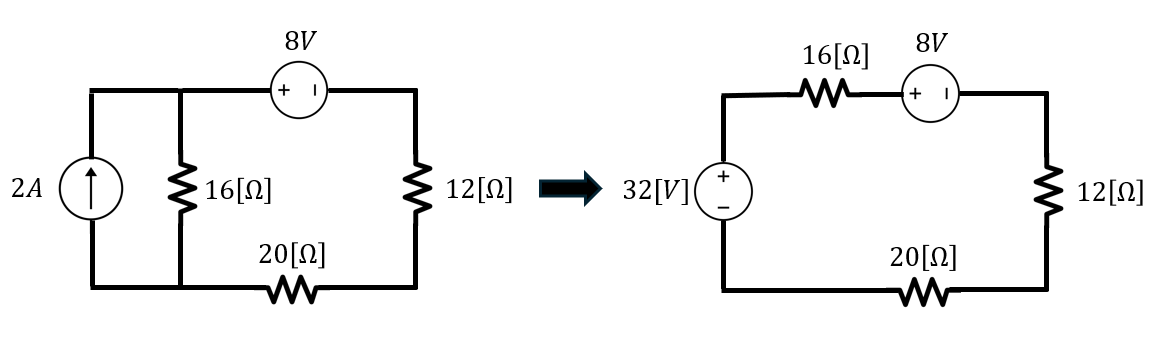
\includegraphics[width=\linewidth]{Auxiliar_3_6}
    \caption{Aproximación con $K=1$ armónico impar.}
  \end{subfigure}
  \hfill
  \begin{subfigure}[t]{0.48\textwidth}
    \centering
    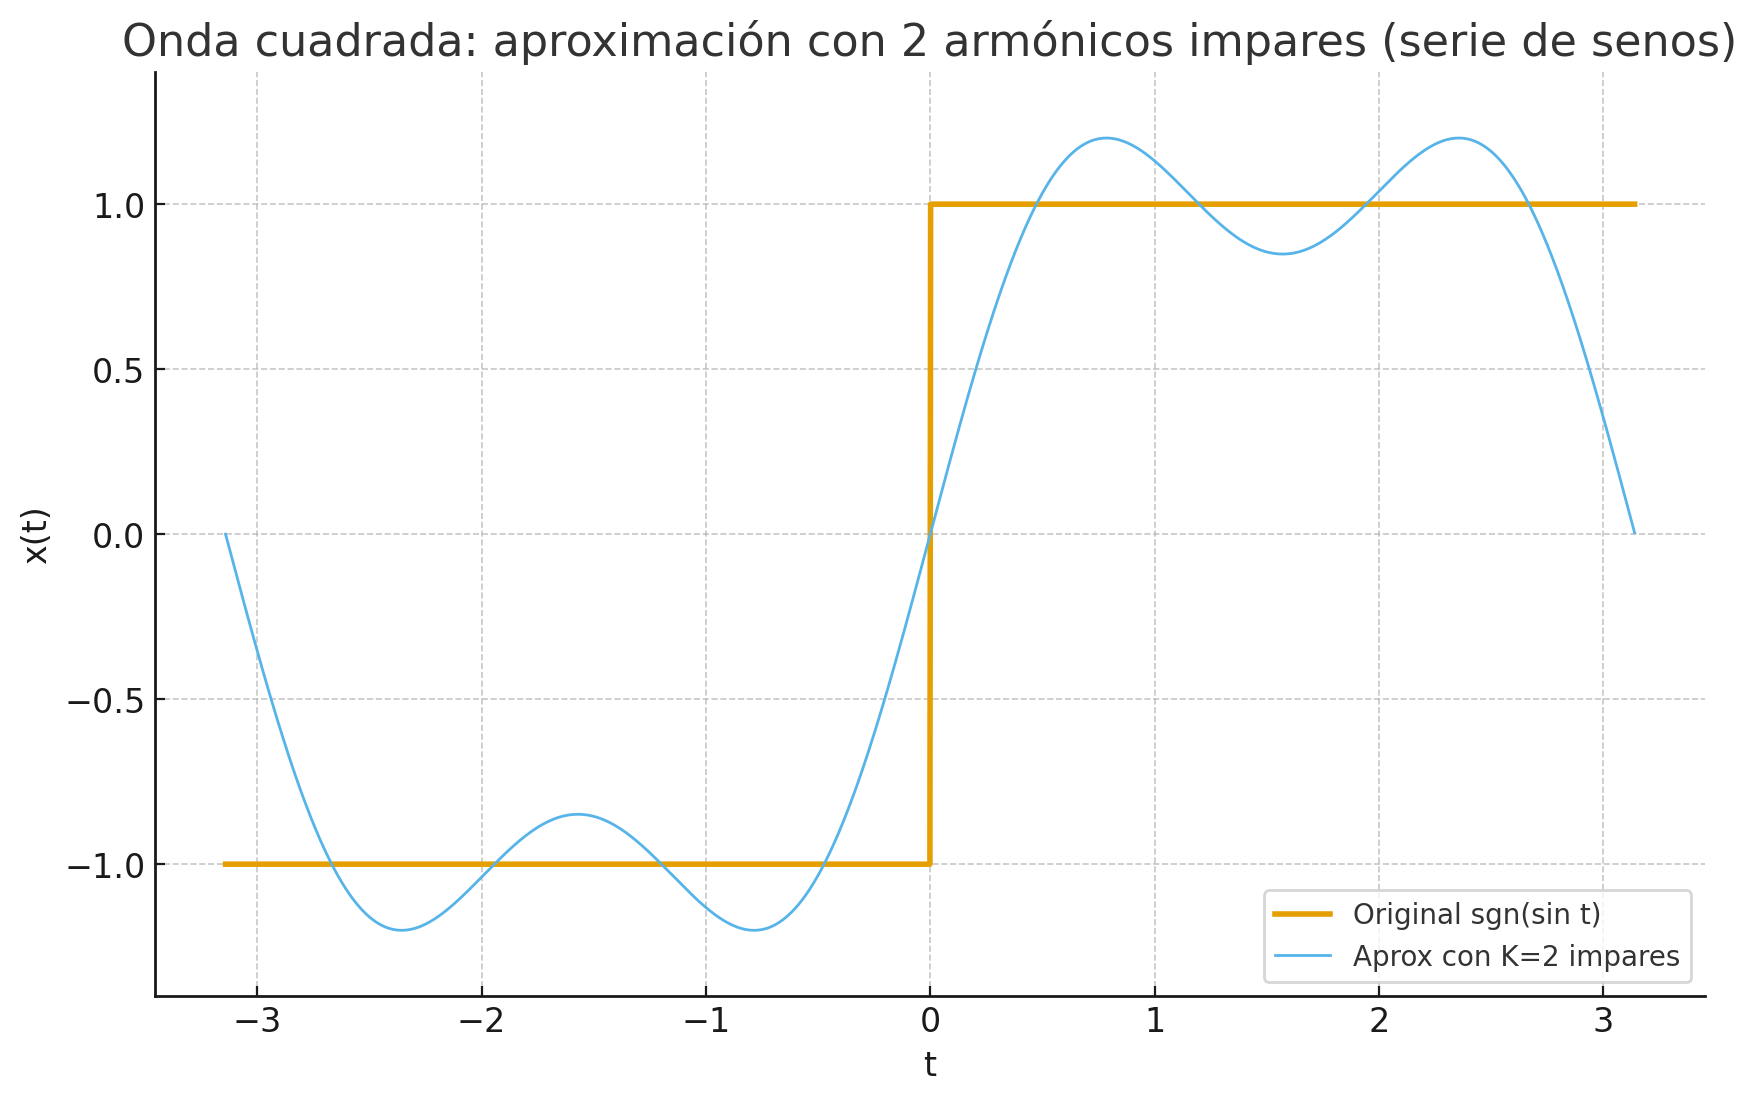
\includegraphics[width=\linewidth]{Auxiliar_3_7}
    \caption{Aproximación con $K=2$ armónicos impares.}
  \end{subfigure}
    
  \begin{subfigure}[t]{0.48\textwidth}
    \centering
    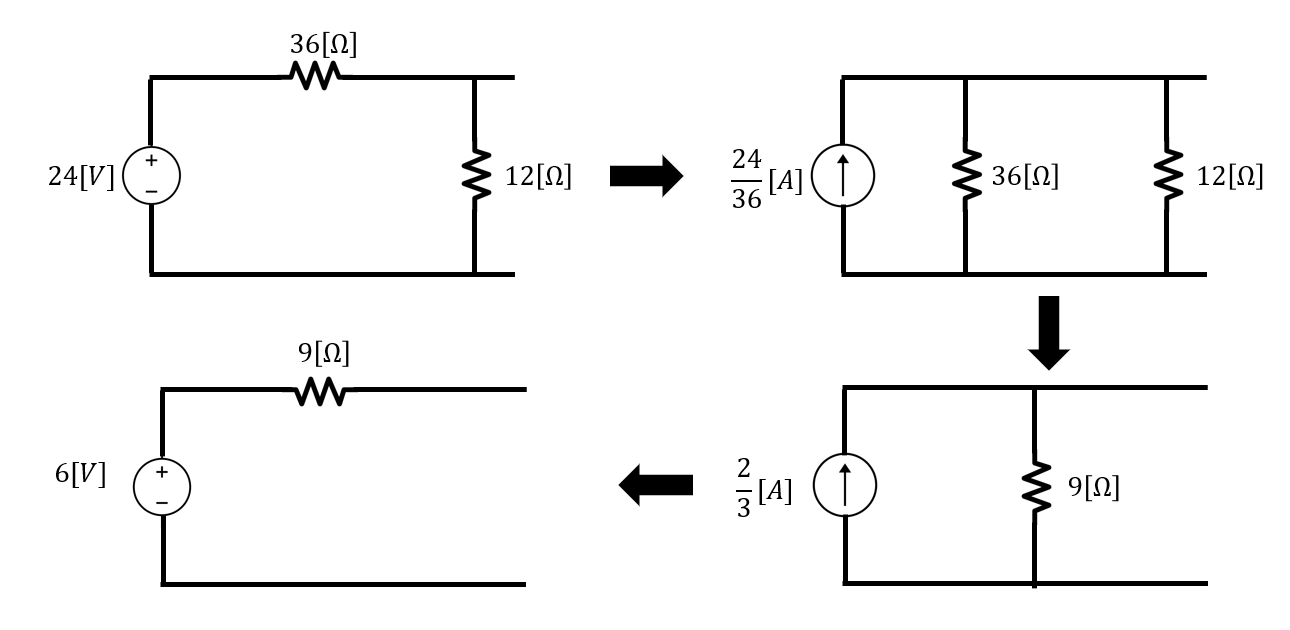
\includegraphics[width=\linewidth]{Auxiliar_3_8}
    \caption{Aproximación con $K=5$ armónicos impares.}
  \end{subfigure}
  \hfill
  \begin{subfigure}[t]{0.48\textwidth}
    \centering
    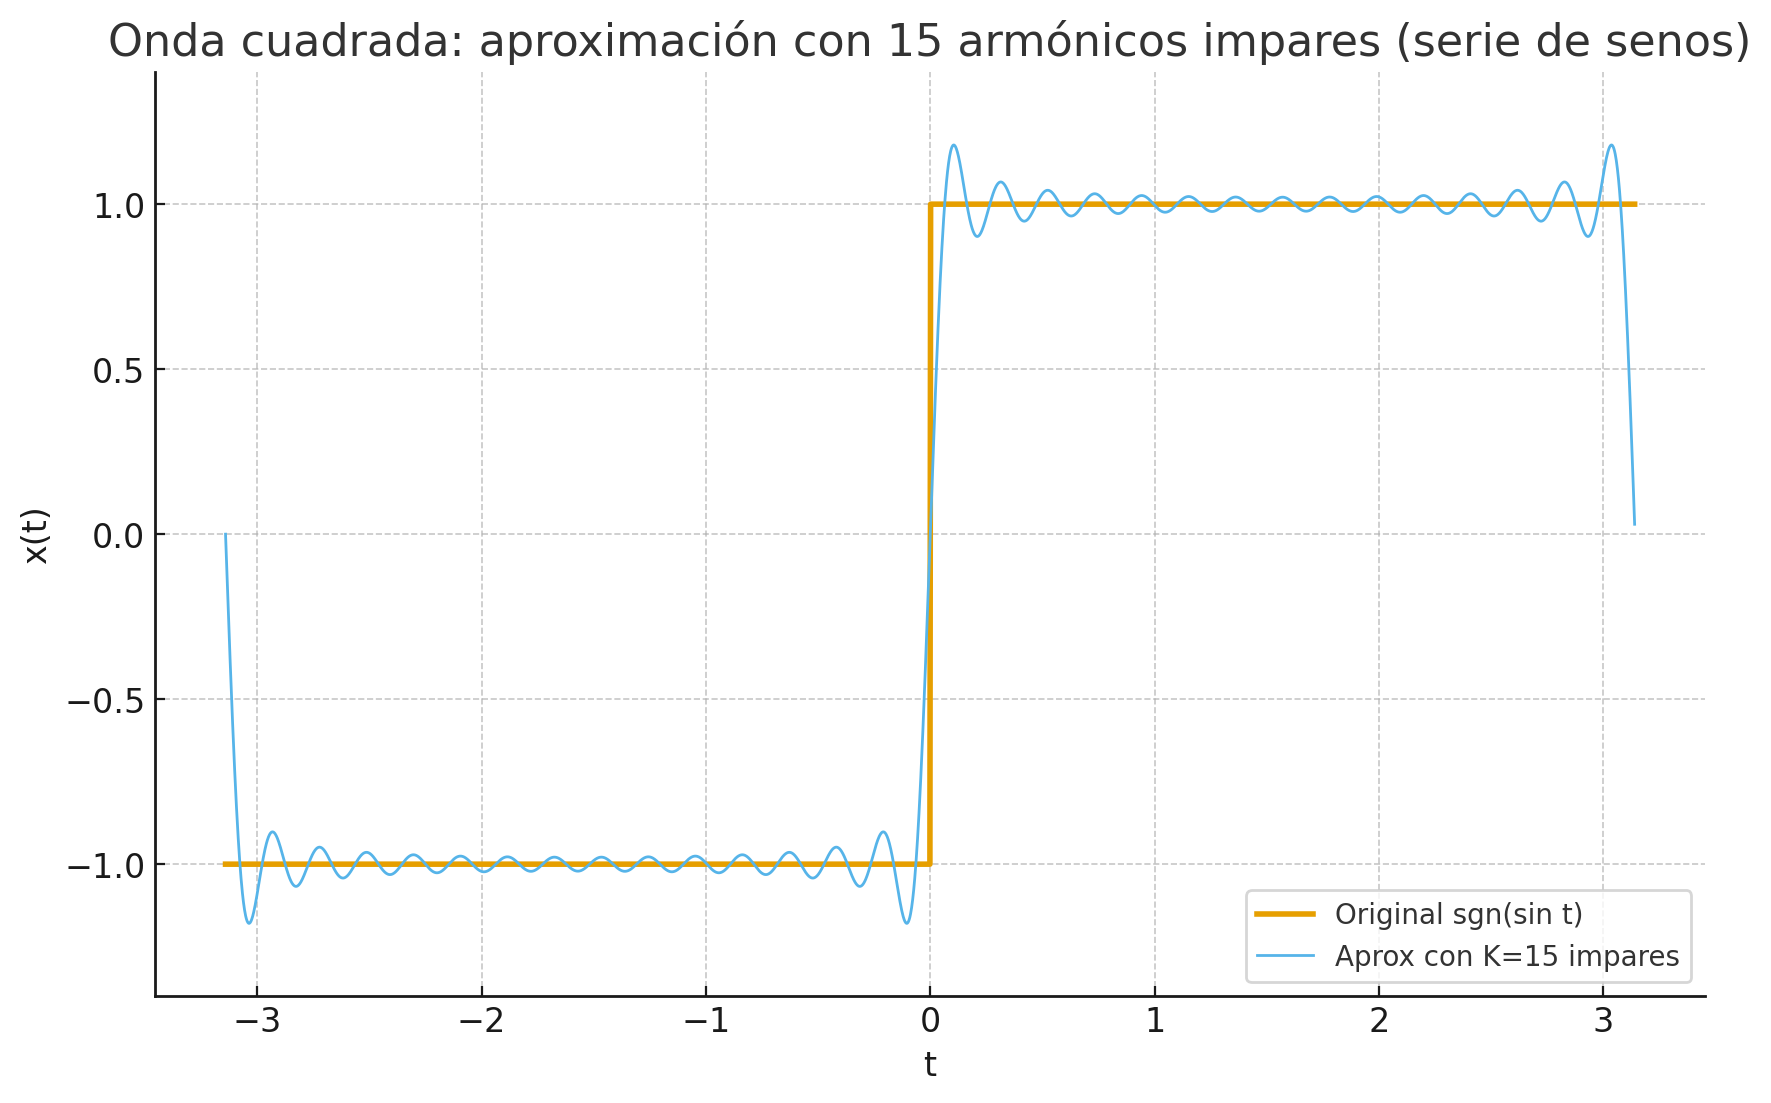
\includegraphics[width=\linewidth]{Auxiliar_3_9}
    \caption{Aproximación con $K=15$ armónicos impares.}
  \end{subfigure}
  \caption{Aproximación de una onda cuadrada mediante la suma de los primeros $K$ armónicos impares (serie de senos). Se observa cómo la aproximación mejora al aumentar $K$, pero aparecen oscilaciones cerca de las discontinuidades (efecto Gibbs).}
  \label{fig:aprox_cuadrada}
\end{figure}

\subsection*{Energía y potencia}
La energía de una señal mide el "contenido total" a lo largo del tiempo:
\begin{equation}
  E_x = \int_{-\infty}^{\infty} |x(t)|^2\,dt
\end{equation}
Para señales periódicas, la energía es infinita, pero se define la potencia promedio en un período:
\begin{equation}
  P_x = \frac{1}{T}\int_{t_0}^{t_0+T} |x(t)|^2\,dt
\end{equation}
La potencia indica cuánta energía se transfiere en promedio por unidad de tiempo.

\subsection*{Relación de Parseval (señales periódicas)}
La relación de Parseval conecta el dominio temporal y el de frecuencias:
\begin{equation}
  P_x = \frac{1}{T}\int_{t_0}^{t_0+T} |x(t)|^2\,dt = \sum_{k=-\infty}^{\infty} |c_k|^2
\end{equation}
Esto permite calcular la potencia directamente a partir de los coeficientes de Fourier, sin necesidad de integrar en el tiempo.\\
\noindent\rule{\textwidth}{0.4pt}
\newpage
%----------------------------
\begin{questions}
%----------------------------
\question
Considere la familia de funciones exponenciales discretas:
\begin{equation}
  A = \left\{ (\gamma_a(n)) \in \mathbb{R}^{\mathbb{N}} : \gamma_a(n) = a^n u(n),\ 0 < a < 1 \right\}
\end{equation}
\begin{enumerate}
  \item Verifique que el impulso discreto $\delta(n)$ puede ser expresado punto a punto como:
  \begin{equation}
    \delta(n) = \gamma_a(n) - a\,\gamma_a(n-1)
  \end{equation}
  \item Del punto anterior, muestre que toda señal discreta $x(n) \in \mathbb{R}^{\mathbb{Z}}$ puede ser descompuesta como:
  \begin{equation}
    x(n) = \sum_{k=-\infty}^{\infty} c_k\,\gamma_a(n-k)
  \end{equation}
  \item Use las propiedades de linealidad e invariancia en el tiempo para expresar la salida $y(n) = \mathcal{T}[x(n)]$ en términos de la entrada $x(n)$ y la señal $g(n) = \mathcal{T}[\gamma_a(n)]$.
\end{enumerate}
%----------------------------
\begin{solution}
\subsection*{Resolución 1.1}
Sea la familia de funciones exponenciales discretas:
\begin{equation}
A = \Big\{ \gamma_a(n) \in \mathbb{R}^{\mathbb{N}} : \gamma_a(n) = a^n u(n), \; 0<a<1 \Big\}.
\end{equation}

Queremos verificar que:
\begin{equation}
\delta(n) = \gamma_a(n) - a\,\gamma_a(n-1).
\end{equation}

Dado que se busca demostrar lo anterior, tendremos lo siguiente:
\begin{align}
\gamma_a(n) - a\,\gamma_a(n-1) &= a^n u(n) - a\cdot a^{n-1}u(n-1) \\
&= a^n u(n) - a^n u(n-1) \\
&= a^n\big[u(n) - u(n-1)\big].
\end{align}

Recordemos que:
\begin{equation}
u(n) - u(n-1) =
\begin{cases}
1, & n=0, \\
0, & n\neq 0,
\end{cases}
\end{equation}
lo cual corresponde exactamente a la definición del impulso discreto \(\delta(n)\). Por lo tanto:
\begin{equation}
\delta(n) = \gamma_a(n) - a\,\gamma_a(n-1).
\end{equation}

\subsection*{Resolución 1.2}
Sabemos que cualquier señal discreta \(x(n)\) puede expresarse como:
\begin{equation}
x(n) = \sum_{k \in \mathbb{Z}} x(k)\,\delta(n-k).
\end{equation}

Sustituyendo la expresión de \(\delta(n)\) obtenida en el punto anterior:
\begin{align}
x(n) &= \sum_{k \in \mathbb{Z}} x(k)\Big[ \gamma_a(n-k) - a\,\gamma_a(n-k-1)\Big] \\
&= \sum_{k \in \mathbb{Z}} x(k)\,\gamma_a(n-k) \;-\; a \sum_{k \in \mathbb{Z}} x(k)\,\gamma_a(n-k-1).
\end{align}

En la segunda suma hacemos el cambio de variable \(k \mapsto k-1\):
\begin{equation}
\sum_{k \in \mathbb{Z}} x(k)\,\gamma_a(n-k-1) 
= \sum_{k \in \mathbb{Z}} x(k-1)\,\gamma_a(n-k).
\end{equation}

Por tanto:
\begin{align}
x(n) &= \sum_{k \in \mathbb{Z}} \Big[x(k) - a\,x(k-1)\Big] \,\gamma_a(n-k).
\end{align}

Definiendo:
\begin{equation}
c_k = x(k) - a\,x(k-1),
\end{equation}
tenemos finalmente:
\begin{equation}
x(n) = \sum_{k \in \mathbb{Z}} c_k\,\gamma_a(n-k).
\end{equation}

\subsection*{Resolución 1.3}
Sea el sistema \( \mathcal{T} \) lineal e invariante en el tiempo (LTI). Definimos:
\begin{equation}
g(n) = \mathcal{T}[\gamma_a(n)].
\end{equation}

La respuesta al impulso del sistema es:
\begin{equation}
h(n) = \mathcal{T}[\delta(n)].
\end{equation}

Usando el resultado de 1.1:
\begin{align}
h(n) &= \mathcal{T}\big[\gamma_a(n) - a\,\gamma_a(n-1)\big] \\
&= \mathcal{T}[\gamma_a(n)] - a\,\mathcal{T}[\gamma_a(n-1)] \\
&= g(n) - a\,g(n-1).
\end{align}

Finalmente, como el sistema es LTI:
\begin{align}
y(n) &= (x * h)(n) \\
&= \sum_{k \in \mathbb{Z}} x(k)\,h(n-k) \\
&= \sum_{k \in \mathbb{Z}} x(k)\Big[g(n-k) - a\,g(n-k-1)\Big].
\end{align}

De este modo:
\begin{equation}
y(n) = \sum_{k \in \mathbb{Z}} x(k)\,\big[g(n-k) - a\,g(n-k-1)\big].
\end{equation}

\end{solution}

%----------------------------
\question Responda lo siguiente:
\begin{enumerate}
  \item Demuestre que
  \begin{equation}
    \frac{1}{T_0} \int_{t_0}^{t_0+T_0} e^{-j 2\pi F_0 \cdot k t} \, dt = 0, \quad \text{si } k \neq 0
  \end{equation}
  siendo $T_0$ el periodo fundamental.

  \item En base a lo anterior demuestre que una señal $x(t)$ periódica de periodo $T_0$, escrita como:
  \begin{equation}
    x(t) = \sum_{k=-\infty}^{\infty} c_k \phi_{k}(t)
  \end{equation}
Los valores de los coeficientes $c_k$ vendrán dados por:
\begin{align}
  c_{k} = \frac{1}{T_0} \langle x(t), \phi_k(t) \rangle &= \frac{1}{T_0} \int_{t_0}^{t_0+T_0} x(t) \phi_k^{*}(t) \, dt
\end{align}
  siendo $\phi_k(t)$ la familia de funciones ortogonales:
  \begin{equation}
    \phi_k(t) = e^{j \frac{2\pi}{T_0} k t}
  \end{equation}
  \item \textbf{[Propuesto]} Finalmente demuestre que:
  \begin{equation}
    \lim_{N \to \infty} \| x(t) - x_N(t) \| = 0 \quad \forall t \in (t_0 , t_0+T_0)
  \end{equation}
  siendo $x_N(t)$ la aproximación de $x(t)$ con $2N+1$ armónicos.
\end{enumerate}
%----------------------------
\begin{solution}
\subsection*{Resolución 2.1}
Se pide el demostrar que:
\begin{equation}
\frac{1}{T_0} \int_{t_0}^{t_0+T_0} e^{-j 2\pi F_0 \cdot k t} \, dt = 0, \quad \text{si } k \neq 0
\end{equation}
Recordando la primitiva de la exponencial compleja, 
\begin{align}
\int e^{at} dt &= \frac{e^{at}}{a} + C, \quad a \neq 0,
\end{align} 
se puede luego demostrar fácilmente evaluando la integral:
\begin{align}
\frac{1}{T_0} \int_{t_0}^{t_0+T_0} e^{-j 2\pi F_0 \cdot k t} \, dt
&= \frac{1}{T_0} \left[ \frac{e^{-j 2\pi F_0 k t}}{-j 2\pi F_0 k} \right]_{t_0}^{t_0+T_0} \\
&= \frac{1}{T_0} \cdot \frac{1}{-j 2\pi F_0 k} \left( e^{-j 2\pi F_0 k (t_0 + T_0)} - e^{-j 2\pi F_0 k t_0} \right) \\
&= \frac{1}{T_0} \cdot \frac{1}{-j 2\pi F_0 k} e^{-j 2\pi F_0 k t_0} \left( e^{-j 2\pi F_0 k T_0} - 1 \right)
\end{align}
Dado que \(F_0 = \frac{1}{T_0}\), tenemos:
\begin{align}
e^{-j 2\pi F_0 k T_0} &= e^{-j 2\pi k} = 1
\end{align}
Por lo tanto:
\begin{align}
\frac{1}{T_0} \int_{t_0}^{t_0+T_0} e^{-j 2\pi F_0 \cdot k t} \, dt &= \frac{1}{T_0} \cdot \frac{1}{-j 2\pi F_0 k} e^{-j 2\pi F_0 k t_0} (1 - 1) = 0
\end{align}
para \(k \neq 0\), como se quería demostrar.
\subsection*{Resolución 2.2}
Dado que podemos escribir la función periódica \(x(t)\) como:
\begin{equation}
x(t) = \sum_{k=-\infty}^{\infty} c_k \phi_{k}(t)
\end{equation}
Luego tenemos que el producto interno entre \(x(t)\) y \(\phi_k(t)\) es:
\begin{align}
\langle x(t), \phi_k(t) \rangle &= \int_{t_0}^{t_0+T_0} x(t) \phi_k^{*}(t) \, dt \\
&= \int_{t_0}^{t_0+T_0} x(t) e^{-j 2\pi F_{0} k t} \, dt \\
&= \int_{t_0}^{t_0+T_0} \left( \sum_{k'=-\infty}^{\infty} c_{k'} \phi_{k'}(t) \right) e^{-j 2\pi F_{0} k t} \, dt \\
&= \sum_{k'=-\infty}^{\infty} c_{k'} \int_{t_0}^{t_0+T_0} e^{j 2\pi F_{0} k' t} \cdot e^{-j 2\pi F_{0} k t} \, dt\\
&= \sum_{k'=-\infty}^{\infty} c_{k'} \int_{t_0}^{t_0+T_0} e^{j 2\pi F_{0} (k' - k) t} \, dt
\end{align}
Como vimos en la resolución 2.1, la integral es cero para \(k' \neq k\) y \(T_0\) para \(k' = k\). Por lo tanto, el producto interno lo podemos escribir en base al impulso como:
\begin{align}
  \sum_{k'=-\infty}^{\infty} c_{k'} \int_{t_0}^{t_0+T_0} e^{j 2\pi F_{0} (k' - k) t} \, dt = \sum_{k'=-\infty}^{\infty} c_{k'} \, \delta(k'-k) T_{0} = c_{k} T_0
\end{align}
Con lo que finalmente tenemos que:
\begin{align}
  \langle x(t), \phi_k(t) \rangle &= c_k T_0 \\
  \Rightarrow \quad c_k &= \frac{1}{T_0} \langle x(t), \phi_k(t) \rangle
\end{align}
De donde se obtiene la expresión buscada para los coeficientes \(c_k\):
\begin{align}
  c_{k} = \frac{1}{T_0} \langle x(t), \phi_k(t) \rangle &= \frac{1}{T_0} \int_{t_0}^{t_0+T_0} x(t) \phi_k^{*}(t) \, dt
\end{align}
\subsection*{Resolución 2.3}
Se pide demostrar que la aproximación por serie de Fourier converge en norma:
\begin{equation}
\lim_{N \to \infty} \| x(t) - x_N(t) \| = 0 \quad \forall t \in (t_0 , t_0+T_0)
\end{equation}

Esta ecuación establece que al incluir más armónicos en la serie de Fourier, el error entre la señal original \(x(t)\) y su aproximación \(x_N(t)\) tiende a cero. Esto garantiza que podemos reconstruir perfectamente cualquier señal usando infinitos armónicos.

La aproximación \(x_N(t)\) usa los primeros \(2N+1\) armónicos (desde \(k=-N\) hasta \(k=N\)):
\begin{equation}
x_N(t) = \sum_{k=-N}^{N} c_k \phi_k(t)
\end{equation}

Para demostrar la convergencia, calculamos la norma \(L^2\) del error en el intervalo \([t_0, t_0+T_0]\):
\begin{align}
\| x(t) - x_N(t) \| &= \sqrt{\langle x(t) - x_N(t), x(t) - x_N(t) \rangle} \\
&= \sqrt{\int_{t_0}^{t_0+T_0} |x(t) - x_N(t)|^2 \, dt}
\end{align}

La clave está en evaluar la integral \(\int_{t_0}^{t_0+T_0} |x(t) - x_N(t)|^2 \, dt\). Usando la identidad \(|a-b|^2 = |a|^2 - 2\text{Re}(ab^*) + |b|^2\), expandimos:
\begin{align}
|x(t) - x_N(t)|^2 &= |x(t)|^2 - 2\text{Re}\{x(t)x_N^*(t)\} + |x_N(t)|^2
\end{align}

Integrando término a término en el intervalo \([t_0, t_0+T_0]\):
\begin{align}
\int_{t_0}^{t_0+T_0} |x(t) - x_N(t)|^2 \, dt &= \int_{t_0}^{t_0+T_0} |x(t)|^2 \, dt - 2\text{Re}\left\{\int_{t_0}^{t_0+T_0} x(t)x_N^*(t) \, dt\right\} + \int_{t_0}^{t_0+T_0} |x_N(t)|^2 \, dt
\end{align}

Ahora analizamos cada integral. Para la integral cruzada, sustituyendo la definición \(x_N(t) = \sum_{k=-N}^{N} c_k \phi_k(t)\):
\begin{align}
\int_{t_0}^{t_0+T_0} x(t)x_N^*(t) \, dt &= \int_{t_0}^{t_0+T_0} x(t) \left( \sum_{k=-N}^{N} c_k^* \phi_k^*(t) \right) dt \\
&= \sum_{k=-N}^{N} c_k^* \int_{t_0}^{t_0+T_0} x(t) \phi_k^*(t) \, dt \\
&= \sum_{k=-N}^{N} c_k^* \cdot c_k T_0 \quad \text{(por la fórmula de análisis: } c_k = \frac{1}{T_0}\int x(t)\phi_k^*(t)dt\text{)} \\
&= T_0 \sum_{k=-N}^{N} |c_k|^2
\end{align}

Para la integral de \(|x_N(t)|^2\), utilizamos la propiedad clave de ortogonalidad de las funciones \(\phi_k(t)\):
\begin{align}
\int_{t_0}^{t_0+T_0} |x_N(t)|^2 \, dt &= \int_{t_0}^{t_0+T_0} \left| \sum_{k=-N}^{N} c_k \phi_k(t) \right|^2 dt \\
&= \sum_{k=-N}^{N} |c_k|^2 T_0 \quad \text{(los términos cruzados se anulan por ortogonalidad)}
\end{align}

Combinando estos resultados en la expresión del error:
\begin{align}
\int_{t_0}^{t_0+T_0} |x(t) - x_N(t)|^2 \, dt &= \int_{t_0}^{t_0+T_0} |x(t)|^2 \, dt - 2 T_0 \sum_{k=-N}^{N} |c_k|^2 + T_0 \sum_{k=-N}^{N} |c_k|^2 \\
&= \int_{t_0}^{t_0+T_0} |x(t)|^2 \, dt - T_0 \sum_{k=-N}^{N} |c_k|^2
\end{align}

Observemos que el término \(-2T_0\sum|c_k|^2 + T_0\sum|c_k|^2 = -T_0\sum|c_k|^2\) muestra que incluir más armónicos efectivamente reduce el error.

Ahora aplicamos la relación de Parseval, que establece que la energía en el dominio temporal es igual a la energía en el dominio de frecuencias:
\begin{equation}
\int_{t_0}^{t_0+T_0} |x(t)|^2 \, dt = T_0 \sum_{k=-\infty}^{\infty} |c_k|^2
\end{equation}

Sustituyendo esta relación en la expresión del error:
\begin{align}
\int_{t_0}^{t_0+T_0} |x(t) - x_N(t)|^2 \, dt &= T_0 \sum_{k=-\infty}^{\infty} |c_k|^2 - T_0 \sum_{k=-N}^{N} |c_k|^2 \\
&= T_0 \sum_{|k|>N} |c_k|^2
\end{align}

Este resultado es fundamental: el error al cuadrado es exactamente \(T_0\) veces la suma de los coeficientes que \textit{no} incluimos en la aproximación (aquellos con \(|k|>N\)). Por tanto, la norma del error viene dada por:
\begin{equation}
\| x(t) - x_N(t) \|^2 = T_0 \sum_{|k|>N} |c_k|^2
\end{equation}

Para que la demostración sea completa, necesitamos que la señal \(x(t)\) tenga energía finita en un período, es decir, que se cumpla \(\sum_{k=-\infty}^{\infty} |c_k|^2 < \infty\). Esta condición es razonable para señales físicamente realizables. Bajo esta hipótesis:
\begin{equation}
\lim_{N \to \infty} \sum_{|k|>N} |c_k|^2 = 0
\end{equation}

puesto que cuando \(N \to \infty\), la suma de los términos "cola" de una serie convergente tiende a cero.

Finalmente, tomando la raíz cuadrada en ambos lados y aplicando el límite:
\begin{equation}
\lim_{N \to \infty} \| x(t) - x_N(t) \| = \lim_{N \to \infty} \sqrt{T_0 \sum_{|k|>N} |c_k|^2} = 0 \quad \forall t \in (t_0, t_0+T_0)
\end{equation}

Esto completa la demostración de que la serie de Fourier converge en norma \(L^2\) hacia la función original. El resultado es poderoso: nos asegura que cualquier señal de energía finita puede ser aproximada arbitrariamente bien mediante una suma finita de armónicos.

\end{solution}
%----------------------------
\question Para la función sinusoidal rectificada mostrada en la figura \ref{fig:aux3_1}, calcule los coeficientes de la serie de Fourier , ademas verifique el cumplimiento del teorema de Parseval.
\begin{figure}[H]
    \centering
    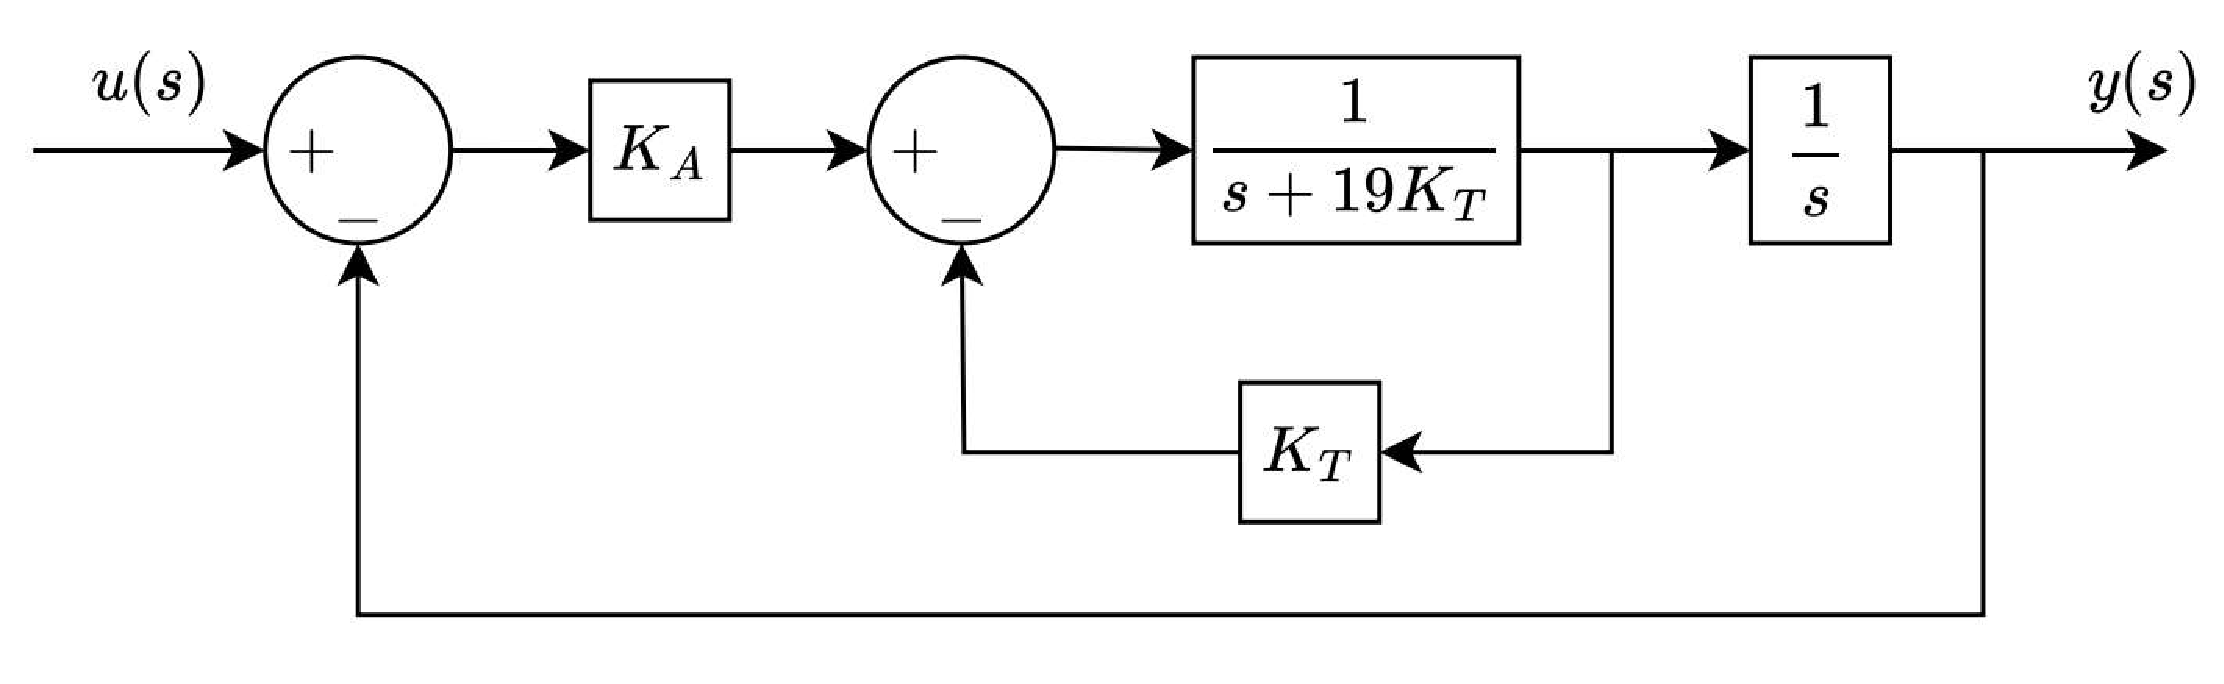
\includegraphics[width=0.6\textwidth]{Auxiliar_3_1}
    \caption{Función sinusoidal rectificada}
    \label{fig:aux3_1}
\end{figure}
%----------------------------
\begin{solution}
  \subsection*{Resolución 3.1}

Sea la sinusoidal rectificada de período \(\tau\) (se extiende periódicamente):
\begin{equation}
x(t)=A\,\sin\!\left(\frac{\pi t}{\tau}\right),\qquad 0\le t<\tau,
\end{equation}
con frecuencia fundamental \(f_0=\tfrac{1}{\tau}\) y pulsación \(\omega_0=\tfrac{2\pi}{\tau}\).
Los coeficientes complejos de Fourier se obtienen con la ecuación de análisis:
\begin{equation}
c_k=\frac{1}{\tau}\int_{0}^{\tau} x(t)\,e^{-jk\omega_0 t}\,dt.
\end{equation}
Sustituyendo \(x(t)\) y usando las identidades de Euler,
\(\sin\theta=\tfrac{e^{j\theta}-e^{-j\theta}}{2j}\), resulta
\begin{align}
c_k
&=\frac{A}{\tau}\int_{0}^{\tau}\sin\!\left(\frac{\pi t}{\tau}\right)e^{-j\frac{2\pi}{\tau}kt}\,dt\\
&=\frac{A}{2j\,\tau}\int_{0}^{\tau}\Big(e^{\,j\frac{\pi}{\tau}(1-2k)t}-e^{-\,j\frac{\pi}{\tau}(1+2k)t}\Big)\,dt\\
&=\frac{A}{2j\,\tau}\left[
\frac{e^{\,j\frac{\pi}{\tau}(1-2k)t}}{j\frac{\pi}{\tau}(1-2k)}
-\frac{e^{-\,j\frac{\pi}{\tau}(1+2k)t}}{-j\frac{\pi}{\tau}(1+2k)}
\right]_{0}^{\tau}.
\end{align}
Como \(e^{j\pi(1-2k)}=e^{-j\pi(1+2k)}=-1\) para todo \(k\in\mathbb{Z}\),
\begin{align}
c_k
&=\frac{A}{2j\,\tau}\left[
\frac{-2}{j\frac{\pi}{\tau}(1-2k)}+\frac{-2}{j\frac{\pi}{\tau}(1+2k)}
\right]
=\frac{A}{\pi}\left(\frac{1}{1-2k}+\frac{1}{1+2k}\right)\\
&=\frac{A}{\pi}\,\frac{(1+2k)+(1-2k)}{1-4k^2}
=\boxed{\;\frac{2A}{\pi\,(1-4k^2)}\;}.
\end{align}
En particular como se tiene que,
\begin{equation}
c_0=\frac{2A}{\pi},\qquad c_{-k}=c_k\quad(\text{coeficientes reales y pares}).
\end{equation}
Dado que los coeficientes son reales, se cumple que \(c_{-k} = c_k^*\). Por otro lado buscamos realizar la verificacion de Parseval, por lo que la potencia promedio en el tiempo es
\begin{align}
P_x
=\frac{1}{\tau}\int_{0}^{\tau}x^2(t)\,dt
=\frac{A^2}{\tau}\int_{0}^{\tau}\sin^2\!\left(\frac{\pi t}{\tau}\right)\,dt
=\frac{A^2}{2}.
\end{align}
En frecuencia,
\begin{align}
\sum_{k=-\infty}^{\infty}|c_k|^2
=\frac{4A^2}{\pi^2}\sum_{k=-\infty}^{\infty}\frac{1}{(1-4k^2)^2}
=\frac{4A^2}{\pi^2}\!\left[\,1+2\sum_{k=1}^{\infty}\frac{1}{(1-4k^2)^2}\right].
\end{align}
Usando la identidad
\begin{equation}
\sum_{k=1}^{\infty}\frac{1}{(1-4k^2)^2}
=\frac{\pi^2}{16}-\frac{1}{2},
\end{equation}
se obtiene
\begin{align}
\sum_{k=-\infty}^{\infty}|c_k|^2
&=\frac{4A^2}{\pi^2}\left[\,1+2\!\left(\frac{\pi^2}{16}-\frac{1}{2}\right)\right]
=\frac{4A^2}{\pi^2}\cdot\frac{\pi^2}{8}
=\frac{A^2}{2}
=P_x,
\end{align}
con lo que queda verificada la relación de Parseval.
\end{solution}
%----------------------------
\question Dadas dos señales $f(t)$ y $g(t)$ con coeficientes de Fourier $c_k$ y $d_k$, respectivamente, encuentre los coeficientes de Fourier de la señal $y(t) = f(t) \cdot g(t)$.
%----------------------------
\begin{solution}
\subsection*{Resolución 4.1}

Este problema aborda una propiedad fundamental de las series de Fourier el cual es el comportamiento de los coeficientes cuando multiplicamos dos señales periódicas.

Consideremos dos señales \(T\)-periódicas \(f(t)\) y \(g(t)\), cada una con su respectiva expansión en serie de Fourier compleja:
\begin{align}
f(t) &= \sum_{k=-\infty}^{\infty} c_k\,e^{jk\omega_0 t}, &
g(t) &= \sum_{m=-\infty}^{\infty} d_m\,e^{jm\omega_0 t}, \qquad \omega_0=\frac{2\pi}{T}.
\end{align}

Aquí \(c_k\) y \(d_m\) son los coeficientes de Fourier de \(f(t)\) y \(g(t)\) respectivamente, y \(\omega_0\) es la frecuencia fundamental. Nuestro objetivo es encontrar los coeficientes de Fourier \(\beta_n\) de la señal producto \(y(t)=f(t)\,g(t)\).

Para calcular estos coeficientes, aplicamos la fórmula estándar de análisis de Fourier:
\begin{equation}
\beta_n=\frac{1}{T}\int_{0}^{T} y(t)\,e^{-jn\omega_0 t}\,dt
= \frac{1}{T}\int_{0}^{T} f(t)\,g(t)\,e^{-jn\omega_0 t}\,dt .
\end{equation}

La clave del desarrollo está en sustituir las expansiones en serie de Fourier de \(f(t)\) y \(g(t)\) directamente en esta integral. Al hacerlo, obtenemos un producto de dos sumas infinitas:
\begin{align}
\beta_n
&= \frac{1}{T}\int_{0}^{T} 
\left(\sum_{k=-\infty}^{\infty} c_k e^{jk\omega_0 t}\right)
\left(\sum_{m=-\infty}^{\infty} d_m e^{jm\omega_0 t}\right)
e^{-jn\omega_0 t}\,dt \\
&= \frac{1}{T}\int_{0}^{T} 
\sum_{k=-\infty}^{\infty}\sum_{m=-\infty}^{\infty} 
c_k d_m e^{j(k+m)\omega_0 t} e^{-jn\omega_0 t}\,dt.
\end{align}

Bajo condiciones apropiadas de convergencia, podemos intercambiar el orden de integración y suma, factorizando los coeficientes constantes:
\begin{align}
\beta_n
&= \sum_{k=-\infty}^{\infty}\sum_{m=-\infty}^{\infty} 
c_k d_m \left(\frac{1}{T}\int_{0}^{T} e^{j(k+m-n)\omega_0 t}\,dt\right).
\end{align}

Ahora aparece la propiedad fundamental de ortogonalidad de las exponenciales complejas. La integral que aparece en paréntesis es:
\begin{equation}
\frac{1}{T}\int_{0}^{T} e^{j\ell\omega_0 t}\,dt
=\begin{cases}
1, & \ell=0,\\
0, & \ell\neq 0,
\end{cases}
\end{equation}
donde \(\ell = k+m-n\). Esta propiedad es crucial porque actúa como un "filtro" que elimina todos los términos excepto aquellos donde \(k+m-n=0\).

La condición \(k+m-n=0\) se puede reescribir como \(m=n-k\). Esto significa que en la doble suma, solo contribuyen los pares \((k,m)\) donde \(m\) tiene esta relación específica con \(k\) y \(n\). Por tanto, la suma sobre \(m\) colapsa y obtenemos:
\begin{align}
\beta_n
&= \sum_{k=-\infty}^{\infty} c_k\, d_{\,n-k}.
\end{align}

En resumen, se demuestra que:
\begin{equation}
\boxed{\;\beta_n=(c*d)_n=\displaystyle\sum_{k=-\infty}^{\infty} c_k\,d_{\,n-k}\;}.
\end{equation}

\end{solution}

%----------------------------
\question Encuentre los coeficientes de Fourier y la serie de Fourier de la función onda cuadrada $f(x)$ definida por:
\begin{equation}
f(x) = \begin{cases}
0 & \text{si } -\pi \leq x < 0 \\
1 & \text{si } 0 \leq x < \pi
\end{cases} \quad \text{y} \quad f(x + 2\pi) = f(x)
\end{equation}
%----------------------------
\begin{solution}
\subsection*{Resolución 5.1}
Buscamos los coeficientes complejos de Fourier \(c_k\) para la función onda cuadrada periódica \(f(x)\) definida por:
\begin{equation}
f(x) = \begin{cases}
0 & \text{si } -\pi \leq x < 0 \\
1 & \text{si } 0 \leq x < \pi
\end{cases} \quad \text{y} \quad f(x + 2\pi) = f(x).
\end{equation}

La función tiene período \(T = 2\pi\), por lo que la frecuencia fundamental es \(\omega_0 = \frac{2\pi}{T} = \frac{2\pi}{2\pi} = 1\).

Los coeficientes complejos de Fourier se calculan usando la fórmula de análisis:
\begin{equation}
c_k = \frac{1}{T}\int_{-\pi}^{\pi} f(x)\,e^{-jkx}\,dx = \frac{1}{2\pi}\int_{-\pi}^{\pi} f(x)\,e^{-jkx}\,dx
\end{equation}

Dado que \(f(x) = 0\) para \(x \in [-\pi, 0)\) y \(f(x) = 1\) para \(x \in [0, \pi)\), tenemos:
\begin{align}
c_k &= \frac{1}{2\pi}\left(\int_{-\pi}^{0} 0 \cdot e^{-jkx}\,dx + \int_{0}^{\pi} 1 \cdot e^{-jkx}\,dx\right) \\
&= \frac{1}{2\pi}\int_{0}^{\pi} e^{-jkx}\,dx
\end{align}

Evaluamos la integral considerando dos casos:
\begin{itemize}
\item Caso 1: \(k = 0\)
\begin{equation}
c_0 = \frac{1}{2\pi}\int_{0}^{\pi} 1\,dx = \frac{1}{2\pi} \cdot \pi = \frac{1}{2}
\end{equation}

\item Caso 2: \(k \neq 0\)
\begin{align}
c_k &= \frac{1}{2\pi}\int_{0}^{\pi} e^{-jkx}\,dx \\
&= \frac{1}{2\pi}\left[\frac{e^{-jkx}}{-jk}\right]_{0}^{\pi} \\
&= \frac{1}{2\pi} \cdot \frac{1}{-jk}\left(e^{-jk\pi} - e^{0}\right) \\
&= \frac{1}{2\pi jk}\left(1 - e^{-jk\pi}\right)
\end{align}
\end{itemize}
Usando la identidad de Euler \(e^{-jk\pi} = \cos(k\pi) - j\sin(k\pi)\), y notando que para \(k\) entero, \(\sin(k\pi) = 0\) y \(\cos(k\pi) = (-1)^k\):
\begin{align}
c_k &= \frac{1}{2\pi jk}\left(1 - (-1)^k\right) \\
&= \begin{cases}
0, & k \text{ par} \\
\frac{1}{\pi jk}, & k \text{ impar}
\end{cases}
\end{align}

Para \(k\) impar, podemos reescribir:
\begin{equation}
c_k = \frac{1}{\pi jk} = -\frac{j}{\pi k} \quad \text{para } k \text{ impar}
\end{equation}

Por tanto, los coeficientes de Fourier son:
\begin{equation}
\boxed{c_k = \begin{cases}
\frac{1}{2}, & k = 0 \\
0, & k \text{ par, } k \neq 0 \\
-\frac{j}{\pi k}, & k \text{ impar}
\end{cases}}
\end{equation}

La serie de Fourier de la onda cuadrada es:
\begin{equation}
\boxed{f(x) = \frac{1}{2} + \sum_{\substack{k=-\infty \\ k \text{ impar}}}^{\infty} \left(-\frac{j}{\pi k}\right)e^{jkx}}
\end{equation}

Alternativamente, usando solo términos positivos y la forma trigonométrica:
\begin{equation}
\boxed{f(x) = \frac{1}{2} + \frac{2}{\pi}\sum_{n=0}^{\infty} \frac{\sin((2n+1)x)}{2n+1}}
\end{equation}

\end{solution}

%----------------------------
\end{questions}
\end{document}